\documentclass[11pt]{article}
\usepackage[margin=1in]{geometry}
\usepackage{amsmath,amssymb,booktabs,graphicx,xcolor}
\usepackage[colorlinks=true,linkcolor=blue!50!black,urlcolor=blue!50!black,citecolor=blue!50!black]{hyperref}
\newcommand{\Cov}{\operatorname{Cov}}
\newcommand{\Var}{\operatorname{Var}}
\newcommand{\E}{\operatorname{E}}
\newcommand{\Kx}{K^{X}}
\newcommand{\Ka}{K^{\rm auto}}
\setlength{\parskip}{4pt}
\setlength{\emergencystretch}{2em}
\newcommand{\chkRM}{$<10^{-6}$}
\newcommand{\chkFisher}{$<10^{-6}$}
\newcommand{\chkSa}{0.5899}
\newcommand{\chkSb}{0.5901}
\newcommand{\chkSc}{0.5903}
\newcommand{\chkHtwo}{0.034}
\newcommand{\chkHtwoRho}{0.0005}


\title{An X-linked additive kernel for the Eftedal et al.\ relative categories}
\author{Derivation and analysis for \texttt{eftedal\_reanalysis} (Phase 2)}
\date{2026-10-20}

\begin{document}
\maketitle

\paragraph{Question.}
The Eftedal et al.\ (2025) correlations split each of 16 relationship types by family side (maternal,
paternal, other) and by the sexes of the pair (ssf, ssm, os), giving 82 categories. Same-sex pairs correlate
slightly more than opposite-sex pairs, and maternal relatives more than paternal ones. The Phase-2 models
need a parameter-free genetic route for such differences. The X chromosome is the obvious candidate: its
inheritance depends on the sexes along the pedigree path. What is its kernel for each category, how does
assortative mating (AM) change it, and how much of the observed differences can it explain?

\paragraph{Answer.}
\begin{enumerate}
  \item \textbf{Kernel.} With full dosage compensation (FDC), the X covariance between relatives is
    proportional to the X kinship $\phi^X$. On the scale of the autosomal kernel, $\Kx=\tfrac43\phi^X$.
    All 82 categories are tabulated, averaging over sexes the data do not record (Table~\ref{tab:kernels}).
  \item \textbf{Size.} X should carry about $s_X\approx2\%$ of $V_A$ (plausible range 1--5\%), not its 5\%
    share of the genome, because under FDC an X locus contributes $3/8$ of an autosomal locus's variance.
  \item \textbf{Assortative mating} does not simply scale the X kernel by the autosomal AM factor; that
    approximation errs by up to $0.75$ in $\Kx$. AM's excess sharing comes from mate correlation on the
    \emph{total} genetic value, and X takes part in it roughly additively, with sex-specific transmission. An
    exact sex-aware path model gives the correction $D_k(m)=\Kx_k(m)-\Ka_k(m)$ on a grid of the mate correlation
    $m$.
  \item \textbf{Signatures.} At $s_X=0.02$, X explains $\le7\%$ of the sibling same-sex excess and of the
    maternal half-sibling excess, with the wrong sex pattern for the latter. It explains about $15$--$35\%$ of
    the small maternal excess among 1st and 2nd cousins, and most of it only at the top of the plausible range.
    It explains $\le3\%$ of the cousins' same-sex excess. Other routes, such as maternal-line or
    sex-specific environment, are needed.
\end{enumerate}
Code and tables are in \texttt{theory/x\_kernel/} (Section~\ref{sec:files}).

\section{The categories and what ``side'' means}\label{sec:side}
Eftedal et al.\ (2025, Fig.~1 legend) define side through the connecting pair one generation above the
relatives. Two women make the pair maternal, two men paternal, and a woman and a man ``other''. Full siblings
are ``other'' because they are connected through both parents. Concretely:

\begin{center}\footnotesize
\begin{tabular}{llll}\toprule
type & maternal & paternal & other\\\midrule
half sibs & shared mother & shared father & --\\
1st cousins & parents are sisters & parents are brothers & brother and sister\\
1st cousins t/uz & parents are twin sisters & twin brothers & --\\
half cousins & parents are half sisters & half brothers & one of each\\
2nd cousins (and t/uz) & parents are two female 1st cousins & two male 1st cousins & one of each\\
co-cousins & connecting mates on both mothers' side & both fathers' side & mixed\\
step sibs & -- & -- & always\\\bottomrule
\end{tabular}
\end{center}

Several sexes are not recorded. These are averaged with equal weights:
\begin{itemize}
  \item the sibling pair at the top of a 2nd-cousin pedigree (FF, FM, MF, MM);
  \item the shared grandparent of half cousins;
  \item the twins' sex for 2nd cousins t/uz;
  \item which member of an os pair is female (this matters only for asymmetric pedigrees).
\end{itemize}
Same-sex twins of unknown zygosity are $\tfrac12$ MZ, $\tfrac12$ DZ, as in our model. Every configuration and
its weight is in \texttt{x\_configs.csv}. Moving any of these weights by 10 percentage points changes $\Kx$ by
at most $0.02$, i.e.\ $\le0.0003$ in correlation. No side definition was ambiguous.

\section{Random mating}\label{sec:rm}
\paragraph{X kinship.} $\phi^X_{ij}$ is the probability that an X allele drawn at random from $i$ and one from
$j$ are identical by descent; a male has one X. The standard recursion runs on the younger member $i$ (who is
not an ancestor of $j$):
\[
\phi^X_{ij}=\begin{cases}\phi^X_{\mathrm{mo}(i),\,j} & i\text{ male}\\[2pt]
\tfrac12\big(\phi^X_{\mathrm{mo}(i),\,j}+\phi^X_{\mathrm{fa}(i),\,j}\big) & i\text{ female}\end{cases},
\qquad \phi^X_{ii}=\begin{cases}1 & \text{male}\\ \tfrac12 & \text{female}\end{cases},
\]
with unrelated founders at $0$. For example, sisters $\tfrac38$, brothers $\tfrac12$, brother--sister
$\tfrac14$. Maternal half siblings are $\tfrac18$ (sisters), $\tfrac12$ (brothers) and $\tfrac14$ (os).
Paternal half sisters are $\tfrac14$, and any paternal half-sibling pair with a male is $0$.

\paragraph{Genetic values and dosage compensation.} Consider one X locus with allele frequency $p$, centred
allele values $u$ ($\Var u=pq$), and effect $b$ per \emph{active} copy.
\begin{itemize}
  \item \emph{FDC} (random X inactivation): a male's value is $b\,u$. A female is a mosaic with value
    $\tfrac b2(u_1+u_2)$. The variances are $b^2pq$ (male) and $b^2pq/2$ (female).
  \item \emph{No dosage compensation (NDC)}: a female's value is $b(u_1+u_2)$, so the variances are $b^2pq$
    (male) and $2b^2pq$ (female).
\end{itemize}
The covariance between relatives is $\sum_{u\in i,\,v\in j}w_uw_v\,pq\,\Pr(u\equiv v)$, with allele weights
$w$. Under FDC ($w=b$ for males, $b/2$ for females) every sex combination gives $\Cov[X_i,X_j]=b^2pq\,
\phi^X_{ij}$. Under NDC ($w=b$ throughout) it gives $4b^2pq\,\phi^X_{ij}\,2^{-\#\text{males}}$.

We put $X$ on the scale of the autosomal kernel by dividing by the \emph{sex-averaged} X variance
$\bar V_X$:
\[
\Cov[X_i,X_j]=\bar V_X\,\Kx_{ij},\qquad
\Kx_{\rm FDC}=\tfrac43\,\phi^X,\qquad \Kx_{\rm NDC}=\tfrac{4}{1.5}\,\phi^X\,2^{-\#\text{males}} .
\]
$\Kx_{ii}$ averages to $1$ over the sexes. MZ females are $\tfrac23$ and MZ males $\tfrac43$ under FDC, which
says only that X variance is twice as large in males. Table~\ref{tab:kernels} gives the kernel for every
biological category. Step siblings, co-cousins and adoptive pairs are $0$ at random mating.

\section{How much of \texorpdfstring{$V_A$}{VA} is X-linked}\label{sec:sx}
\begin{itemize}
  \item \textbf{FDC is supported.} Sidorenko et al.\ (2019) estimate a male/female ratio of X-linked
    $h^2_{\rm SNP}$ of $1.9$--$2.2$ across 20 UK Biobank traits (FDC predicts 2, NDC $\tfrac12$).
  \item \textbf{Per-length expectation.} X is 5.0\% of the haploid genome (156 of about 3{,}100\,Mb), and
    about 4\% of protein-coding genes. An autosomal locus with per-allele effect $b$ contributes $2b^2pq$.
    Under FDC an X locus with the same per-active-copy effect contributes $b^2pq$ in males and $b^2pq/2$ in
    females, so $3/8$ of an autosomal locus on average. Hence
    \[
    s_X=\frac{0.05\times\tfrac38}{0.95+0.05\times\tfrac38}\approx0.019\qquad(\text{NDC: }\approx0.038).
    \]
  \item \textbf{Empirical check.} In UK Biobank, X explains $0.63\%$ (males) and $0.30\%$ (females) of
    phenotypic variance on average. That is roughly 1--3\% of the traits' total $h^2_{\rm SNP}$, and lower per
    Mb than the autosomes, as haploidy predicts (Sidorenko et al.\ 2019).
  \item \textbf{Recommendation.} Fix $s_X=0.02$, with plausible range $0.01$--$0.05$. The upper end allows for
    enrichment of brain and intellectual-disability genes on X and for partial escape from X inactivation.
\end{itemize}

\section{Assortative mating}\label{sec:am}
\paragraph{Sex-aware model.} Each person carries an autosomal value $A^a$ and an X value $X$, with $A=A^a+X$
and $Y=A+E$. Under FDC, writing $V_{X\!f0}$ for the base female X variance (the male one is $2V_{X\!f0}$):
\[
\begin{aligned}
A^a_o&=\tfrac12\big(A^a_{\rm mo}+A^a_{\rm fa}\big)+e^a, & \Var e^a&=\tfrac12V_{a0},\\
X_{\rm daughter}&=\tfrac12X_{\rm mo}+\tfrac12X_{\rm fa}+e_d, & \Var e_d&=\tfrac14V_{X\!f0},\\
X_{\rm son}&=X_{\rm mo}+e_s, & \Var e_s&=V_{X\!f0}.
\end{aligned}
\]
A son's X value is his mother's transmitted allele counted at full male dosage, so it regresses on her value
with coefficient $1$ and on his father's with $0$. Segregation variances keep their random-mating values, as
in Fisher's treatment. Mates are matched on $Y$ with correlation $\rho_y$ (Gaussian assortment), so for the
vector $z=(A^a,X)$
\[
\Cov[z_{\rm mo},z_{\rm fa}]=\rho_y\,\Sigma_F\mathbf 1\mathbf 1^{\!\top}\Sigma_M/(\sigma_{Y\!F}\sigma_{Y\!M}),
\]
and the per-sex covariance matrices $\Sigma_F,\Sigma_M$ are iterated to equilibrium. The genotypic mate
correlation is $m=\operatorname{Corr}[A_{\rm mo},A_{\rm fa}]$. For each category the stationary model is built
in pathMgr over its pedigree configurations, with one co-path per union. This includes the childless unions
that connect step siblings and co-cousins.

\paragraph{Definition used by the model.} At matched $m$, run the model with an X share $s$ and without
($s=0$, giving $\Ka_k(m)$), and define $\Kx$ by the decomposition the Phase-2 model uses:
\[
K^{\rm total}_k(m)=(1-s)\,\Ka_k(m)+s\,\Kx_k(m)
\quad\Longleftrightarrow\quad
K^{\rm total}_k(m)=\Ka_k(m)+s\,D_k(m),
\]
with $D_k=\Kx_k-\Ka_k$.
$\Kx$ absorbs the A--X cross covariances that AM creates; they are first order in $s$.

\paragraph{Checks.}
\begin{itemize}
  \item At $m=0$ the model reproduces the closed forms of Section~\ref{sec:rm} for all 82 categories (max
    error \chkRM).
  \item The autosomal part reproduces Fisher's sibling kernel $(1+m)/2$ (max error \chkFisher).
  \item $\Kx$ does not depend on $s$: opposite-sex siblings at $m=0.43$ give \chkSa, \chkSb\ and \chkSc\ at
    $s=0.005,0.02,0.05$.
  \item At fixed $m$, changing $h^2$ from $0.5$ to $0.78$ moves $D$ by at most \chkHtwo, i.e.\
    $\le\chkHtwoRho$ in correlation.
\end{itemize}

\paragraph{Results.} Figure~\ref{fig:D} and Table~\ref{tab:am} show $D_k(m)$.
\begin{enumerate}
  \item \textbf{Siblings: AM shrinks the correction.} From $m=0$ to $m=0.43$, $D$ goes from $+0.17$ to $+0.04$
    for brothers and from $-0.17$ to $-0.13$ for opposite-sex pairs, because AM-induced sharing is common to X
    and autosomes.
  \item \textbf{AM widens the side contrast for distant relatives.} Paternal-side cousin pairs that include a
    male cannot share X through the father--son link, yet the autosomal excess grows with $m$, so their $D$
    becomes more negative. Maternal-side pairs keep their advantage, because mother-to-son X transmission has
    coefficient $1$. The maternal$-$paternal contrast in $D$ grows from $0.24$ to $0.34$ for 1st cousins and
    from $0.06$ to $0.18$ for 2nd cousins.
  \item \textbf{In-laws acquire small corrections}, e.g.\ $D=-0.11$ for paternal co-cousins, both male. Their
    autosomal kernel is pure AM, and X reaches them through the same sex-specific transmission.
\end{enumerate}

\paragraph{Approximations.} Table~\ref{tab:approx} compares two shortcuts with the exact $\Kx$.
\begin{itemize}
  \item \emph{Autosomal AM factor on the random-mating X kernel},
    $\Kx(0)\,\Ka(m)/\Ka(0)$, is poor. It treats X's AM excess as proportional to its random-mating sharing,
    so it gives zero excess to every pair with $\phi^X=0$, which is wrong.
  \item \emph{A constant correction}, $D_k(m)\approx D_k(0)=\Kx_{\rm FDC}-a_k$, errs by $\le0.002$ in
    correlation at $s_X=0.02$, $V_A=0.5$. It is acceptable if interpolation is inconvenient.
\end{itemize}

\section{GxG, mtDNA and Y}
\begin{itemize}
  \item \textbf{GxG.} No X version of the $a^2$ kernel is needed. Pairs involving X carry about $2s_X\approx4\%$
    of GxG variance, and replacing $a$ by the X kernel for them moves the GxG kernel by $\lesssim0.01$, i.e.\
    $\le0.002$ in correlation.
  \item \textbf{mtDNA} acts as a maternal-line indicator (column \texttt{mt} of Table~\ref{tab:kernels}): 1 for
    siblings, maternal half siblings and maternal 1st cousins; $\tfrac12$ for maternal half cousins; $\tfrac14$
    for maternal 2nd cousins. Its variance for cognitive traits is expected to be negligible, and the
    indicator is confounded with any maternal-line environment.
  \item \textbf{Y} is shared only by paternal-line male pairs; it is ignored (\texttt{y\_share} in
    \texttt{x\_kinship.csv}).
\end{itemize}

\section{Predicted signatures against the data}\label{sec:sig}
X adds $V_A\,s_X\,D_k(m)$ to the correlation of category $k$. Contrasts are formed identically for the data
and for the prediction:
\begin{itemize}
  \item same-sex minus opposite-sex: per side, $\tfrac12(\mathrm{ssf}+\mathrm{ssm})-\mathrm{os}$, then
    averaged over sides;
  \item maternal minus paternal: per sex composition, then averaged.
\end{itemize}
Observed standard errors assume independent category estimates. Table~\ref{tab:sig} and
Figure~\ref{fig:sig} use $m=0.43$.

\begin{enumerate}
  \item \textbf{Siblings and half siblings: X is far too small.} It accounts for $\le7\%$ of the sibling
    same-sex excess ($0.030$) and of the maternal half-sibling excess ($0.050$), and $\le18\%$ even at
    $s_X=0.05$. The sex pattern also disagrees. X puts the maternal half-sibling excess in brothers ($+0.005$)
    and opposite-sex pairs ($+0.003$), with sisters slightly \emph{paternal} ($-0.0005$). The data show the
    excess in all three compositions (ssf $+0.035$, ssm $+0.062$, os $+0.052$).
  \item \textbf{Cousins' maternal excess: X can contribute.} It accounts for about $15$--$35\%$ of the 1st- and
    2nd-cousin excess ($0.014$ and $0.0095$) at central values, and most of it only at $s_X=0.05$, $V_A=0.7$.
  \item \textbf{Cousins' same-sex excess: X is negligible} ($\le3\%$).
  \item \textbf{Half cousins} show a paternal excess ($-0.013\pm0.011$), the opposite of X's prediction, but
    the observed value is within about $1.5$ SE of it.
  \item \textbf{No dosage compensation} changes the predicted contrasts by at most a factor of $2.5$ and leaves
    every conclusion unchanged (\texttt{signatures.csv}).
\end{enumerate}

\section{Implications for the Phase-2 model}
\begin{enumerate}
  \item Use $K^{\rm total}_k(m)=\Ka_k(m)+s_X\,D_k(m)$. Keep our own $\Ka$ (Nagylaki half siblings, corrected
    step siblings, and so on), and interpolate $D_k$ linearly in $m$ from \texttt{x\_kernel\_grid.csv}.
  \item Fix $s_X=0.02$, and report sensitivity at $0.05$. Estimating $s_X$ freely would mainly absorb the
    environmental side and sex effects that X cannot produce.
  \item Expect X to change fitted sex and side multipliers only slightly. Its largest per-category effect is
    $\le0.005$ in correlation.
\end{enumerate}

\paragraph{Caveats.}
\begin{itemize}
  \item The model assumes primary phenotypic AM with Gaussian assortment at equilibrium, unlinked loci, no
    escape from X inactivation and no sex-specific autosomal effects.
  \item The 2nd cousins / other / ssf row is a suspected duplicate (\texttt{data/README.md}). It enters only
    the 2nd-cousin same-sex contrast.
  \item The equal sex weights could be replaced by registry frequencies, but the effect is negligible
    (Section~\ref{sec:side}).
\end{itemize}

\begin{figure}[!tbp]\centering
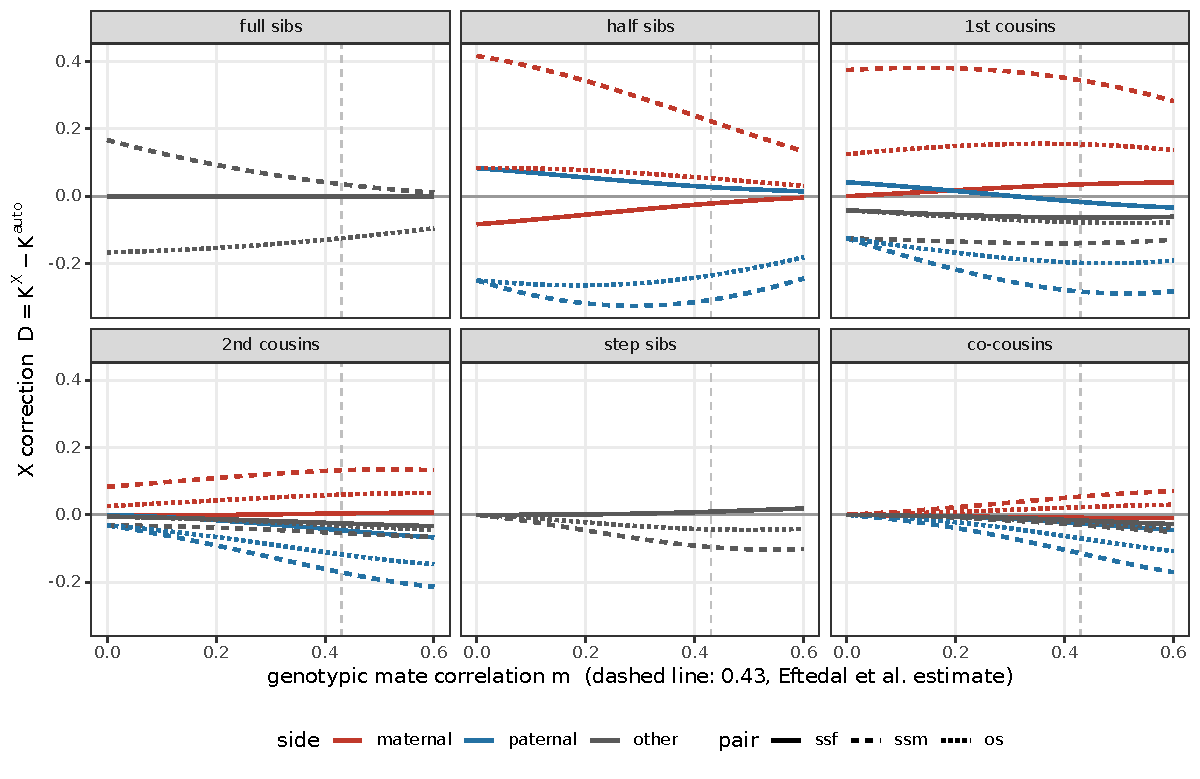
\includegraphics[width=\linewidth]{fig/D_vs_m.pdf}
\caption{The X correction $D=\Kx-\Ka$ against the genotypic mate correlation $m$ (exact, FDC). The effect on a
correlation is $V_A\,s_X\,D$: about $0.01\,D$ at $s_X=0.02$, $V_A=0.5$.}\label{fig:D}
\end{figure}

\begin{figure}[!tbp]\centering
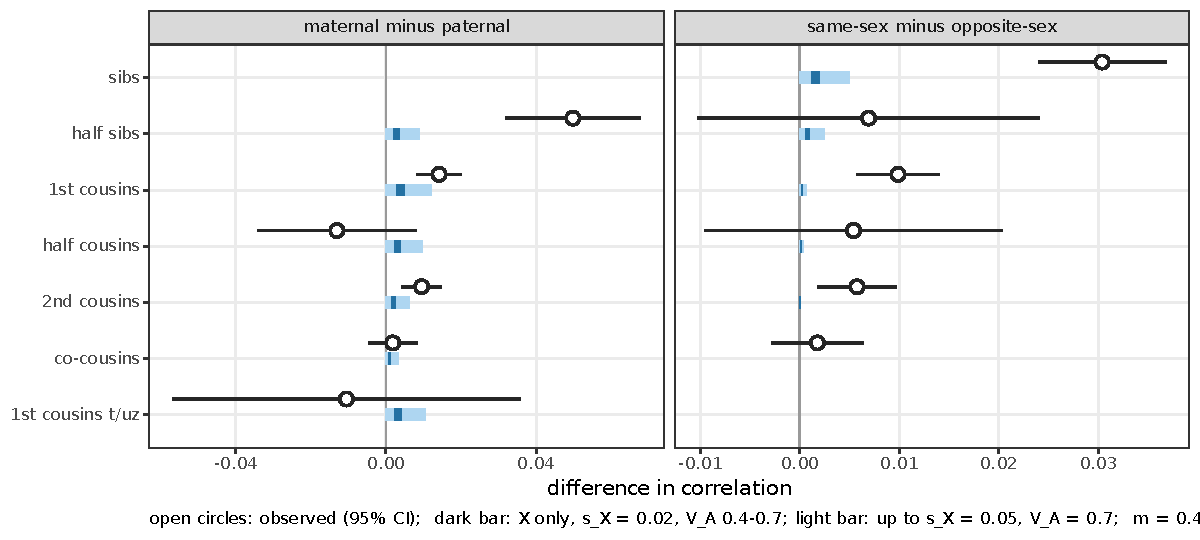
\includegraphics[width=\linewidth]{fig/signatures.pdf}
\caption{Observed contrasts (open circles, 95\% CI) against X alone (bars), at $m=0.43$.}\label{fig:sig}
\end{figure}

\begin{table}[!tbp]\centering\footnotesize
\caption{Predicted X-only contrasts against the data. ``Explained'' is the prediction at $s_X=0.02$, $V_A=0.7$
as a share of the observed contrast, shown where the observed contrast is beyond 2 SE.}\label{tab:sig}
\begin{tabular}{ll|rr|rr|r}\toprule
 & & \multicolumn{2}{c|}{observed} & \multicolumn{2}{c|}{X only, $m=0.43$} & \\
contrast & type & estimate & SE & $s_X{=}0.02$, $V_A$ 0.4--0.7 & $s_X{=}0.05$, $V_A{=}0.7$ & explained\\\midrule
ss $-$ os & dz & -0.0305 & 0.0342 & +0.0011 -- +0.0020 & +0.0050 & n.s. \\
ss $-$ os & sibs & +0.0304 & 0.0033 & +0.0011 -- +0.0020 & +0.0050 & 7\% \\
ss $-$ os & half sibs & +0.0069 & 0.0088 & +0.0006 -- +0.0010 & +0.0025 & n.s. \\
ss $-$ os & 1st cousins & +0.0099 & 0.0021 & +0.0002 -- +0.0003 & +0.0007 & 3\% \\
ss $-$ os & half cousins & +0.0054 & 0.0076 & +0.0001 -- +0.0001 & +0.0003 & n.s. \\
ss $-$ os & 2nd cousins & +0.0058 & 0.0020 & 0.0000 -- +0.0001 & +0.0001 & $<$1\% \\
ss $-$ os & step sibs & +0.0137 & 0.0197 & 0.0000 -- 0.0000 & 0.0000 & n.s. \\
ss $-$ os & cocousins & +0.0018 & 0.0023 & 0.0000 -- 0.0000 & 0.0000 & n.s. \\
mat $-$ pat & half sibs & +0.0498 & 0.0092 & +0.0021 -- +0.0036 & +0.0090 & 7\% \\
mat $-$ pat & 1st cousins & +0.0142 & 0.0030 & +0.0027 -- +0.0048 & +0.0120 & 34\% \\
mat $-$ pat & half cousins & -0.0131 & 0.0108 & +0.0022 -- +0.0039 & +0.0098 & n.s. \\
mat $-$ pat & 2nd cousins & +0.0095 & 0.0028 & +0.0014 -- +0.0025 & +0.0062 & 26\% \\
mat $-$ pat & 1st cousins t/uz & -0.0105 & 0.0237 & +0.0024 -- +0.0042 & +0.0105 & n.s. \\
mat $-$ pat & cocousins & +0.0018 & 0.0033 & +0.0007 -- +0.0013 & +0.0032 & n.s. \\
\bottomrule\end{tabular}

\end{table}

\begin{table}[!tbp]\centering\small
\caption{Exact $\Kx$ and $D$ under AM for selected categories (FDC).}\label{tab:am}
\begin{tabular}{ll|rr|rr|rr}\toprule
 & & \multicolumn{2}{c|}{$m=0$} & \multicolumn{2}{c|}{$m=0.2$} & \multicolumn{2}{c}{$m=0.43$}\\
category & sex & $K^X$ & $D$ & $K^X$ & $D$ & $K^X$ & $D$\\\midrule
sibs, other & ssf & 0.500 & 0.000 & 0.600 & 0.000 & 0.715 & 0.000 \\
sibs, other & ssm & 0.667 & 0.167 & 0.693 & 0.093 & 0.751 & 0.036 \\
sibs, other & os & 0.333 & -0.167 & 0.446 & -0.154 & 0.590 & -0.125 \\
half sibs, maternal & ssf & 0.167 & -0.083 & 0.313 & -0.055 & 0.516 & -0.022 \\
half sibs, maternal & ssm & 0.667 & 0.417 & 0.711 & 0.343 & 0.760 & 0.223 \\
half sibs, maternal & os & 0.333 & 0.083 & 0.445 & 0.077 & 0.591 & 0.053 \\
half sibs, paternal & ssf & 0.333 & 0.083 & 0.424 & 0.056 & 0.565 & 0.027 \\
half sibs, paternal & ssm & 0.000 & -0.250 & 0.049 & -0.319 & 0.229 & -0.308 \\
half sibs, paternal & os & 0.000 & -0.250 & 0.103 & -0.265 & 0.302 & -0.235 \\
1st cousins, maternal & ssf & 0.125 & 0.000 & 0.234 & 0.018 & 0.401 & 0.035 \\
1st cousins, maternal & ssm & 0.500 & 0.375 & 0.596 & 0.380 & 0.710 & 0.344 \\
1st cousins, maternal & os & 0.250 & 0.125 & 0.365 & 0.149 & 0.520 & 0.155 \\
1st cousins, paternal & ssf & 0.167 & 0.042 & 0.232 & 0.016 & 0.349 & -0.017 \\
1st cousins, paternal & ssm & 0.000 & -0.125 & -0.002 & -0.218 & 0.082 & -0.284 \\
1st cousins, paternal & os & 0.000 & -0.125 & 0.048 & -0.168 & 0.168 & -0.198 \\
1st cousins, other & ssf & 0.083 & -0.042 & 0.161 & -0.055 & 0.302 & -0.064 \\
1st cousins, other & ssm & 0.000 & -0.125 & 0.081 & -0.135 & 0.226 & -0.140 \\
1st cousins, other & os & 0.083 & -0.042 & 0.154 & -0.062 & 0.288 & -0.078 \\
2nd cousins, maternal & ssf & 0.029 & -0.003 & 0.077 & -0.001 & 0.191 & 0.004 \\
2nd cousins, maternal & ssm & 0.115 & 0.083 & 0.187 & 0.109 & 0.319 & 0.133 \\
2nd cousins, maternal & os & 0.057 & 0.026 & 0.121 & 0.043 & 0.247 & 0.060 \\
2nd cousins, paternal & ssf & 0.031 & 0.000 & 0.062 & -0.016 & 0.141 & -0.046 \\
2nd cousins, paternal & ssm & 0.000 & -0.031 & -0.013 & -0.091 & 0.016 & -0.171 \\
2nd cousins, paternal & os & 0.000 & -0.031 & 0.012 & -0.066 & 0.069 & -0.118 \\
step sibs, other & ssf & 0.000 & 0.000 & 0.094 & 0.001 & 0.311 & 0.009 \\
step sibs, other & ssm & 0.000 & 0.000 & 0.046 & -0.046 & 0.206 & -0.096 \\
step sibs, other & os & 0.000 & 0.000 & 0.070 & -0.022 & 0.258 & -0.043 \\
cocousins, maternal & ssf & 0.000 & 0.000 & 0.021 & -0.004 & 0.104 & -0.009 \\
cocousins, maternal & ssm & 0.000 & 0.000 & 0.048 & 0.022 & 0.167 & 0.054 \\
cocousins, maternal & os & 0.000 & 0.000 & 0.035 & 0.009 & 0.135 & 0.023 \\
cocousins, paternal & ssf & 0.000 & 0.000 & 0.021 & -0.005 & 0.088 & -0.025 \\
cocousins, paternal & ssm & 0.000 & 0.000 & -0.013 & -0.039 & -0.002 & -0.115 \\
cocousins, paternal & os & 0.000 & 0.000 & 0.004 & -0.022 & 0.042 & -0.070 \\
\bottomrule\end{tabular}

\end{table}

\begin{table}[!tbp]\centering\small
\caption{Approximation errors against the exact $\Kx$ over the 58 biological categories.
$|\Delta\rho|$ is the error in correlation at $s_X=0.02$, $V_A=0.5$.}\label{tab:approx}
\begin{tabular}{rl|rr|r}\toprule
$m$ & approximation & median $|\Delta K^X|$ & max $|\Delta K^X|$ & max $|\Delta\rho|$\\\midrule
0.2 & constant $D$: $K^X(0)+K^{auto}(m)-a$ & 0.025 & 0.093 & 0.0009 \\
0.2 & AM factor: $K^X(0)\,K^{auto}(m)/a$ & 0.046 & 0.271 & 0.0027 \\
0.43 & constant $D$: $K^X(0)+K^{auto}(m)-a$ & 0.049 & 0.194 & 0.0019 \\
0.43 & AM factor: $K^X(0)\,K^{auto}(m)/a$ & 0.136 & 0.752 & 0.0075 \\
\bottomrule\end{tabular}

\end{table}

\begin{table}[!tbp]\centering\small
\caption{Random-mating X kernels for the biological categories. $a$ is autosomal relatedness, FDC is
$\tfrac43\phi^X$, NDC the alternative convention, and mt the probability of sharing mtDNA.}\label{tab:kernels}
\begin{tabular}{lr|rrr|rrr|r}\toprule
 & & \multicolumn{3}{c|}{FDC (default)} & \multicolumn{3}{c|}{NDC} & \\
category & $a$ & ssf & ssm & os & ssf & ssm & os & mt\\\midrule
mz & 1.000 & 0.667 & 1.333 & -- & 1.333 & 0.667 & -- & 1.00 \\
uz & 0.750 & 0.583 & 1.000 & -- & 1.167 & 0.500 & -- & 1.00 \\
dz & 0.500 & 0.500 & 0.667 & 0.333 & 1.000 & 0.333 & 0.333 & 1.00 \\
sibs & 0.500 & 0.500 & 0.667 & 0.333 & 1.000 & 0.333 & 0.333 & 1.00 \\
half sibs, maternal & 0.250 & 0.167 & 0.667 & 0.333 & 0.333 & 0.333 & 0.333 & 1.00 \\
half sibs, paternal & 0.250 & 0.333 & 0.000 & 0.000 & 0.667 & 0.000 & 0.000 & 0.00 \\
1st cousins t/uz, maternal & 0.188 & 0.146 & 0.583 & 0.292 & 0.292 & 0.292 & 0.292 & 1.00 \\
1st cousins t/uz, paternal & 0.188 & 0.250 & 0.000 & 0.000 & 0.500 & 0.000 & 0.000 & 0.00 \\
1st cousins, maternal & 0.125 & 0.125 & 0.500 & 0.250 & 0.250 & 0.250 & 0.250 & 1.00 \\
1st cousins, paternal & 0.125 & 0.167 & 0.000 & 0.000 & 0.333 & 0.000 & 0.000 & 0.00 \\
1st cousins, other & 0.125 & 0.083 & 0.000 & 0.083 & 0.167 & 0.000 & 0.083 & 0.00 \\
half cousins, maternal & 0.062 & 0.062 & 0.250 & 0.125 & 0.125 & 0.125 & 0.125 & 0.50 \\
half cousins, paternal & 0.062 & 0.083 & 0.000 & 0.000 & 0.167 & 0.000 & 0.000 & 0.00 \\
half cousins, other & 0.062 & 0.042 & 0.000 & 0.042 & 0.083 & 0.000 & 0.042 & 0.00 \\
2nd cousins t/uz, maternal & 0.047 & 0.049 & 0.198 & 0.099 & 0.099 & 0.099 & 0.099 & 0.50 \\
2nd cousins t/uz, paternal & 0.047 & 0.073 & 0.000 & 0.000 & 0.146 & 0.000 & 0.000 & 0.00 \\
2nd cousins t/uz, other & 0.047 & 0.036 & 0.000 & 0.036 & 0.073 & 0.000 & 0.036 & 0.00 \\
2nd cousins, maternal & 0.031 & 0.029 & 0.115 & 0.057 & 0.057 & 0.057 & 0.057 & 0.25 \\
2nd cousins, paternal & 0.031 & 0.031 & 0.000 & 0.000 & 0.062 & 0.000 & 0.000 & 0.00 \\
2nd cousins, other & 0.031 & 0.026 & 0.000 & 0.026 & 0.052 & 0.000 & 0.026 & 0.00 \\
\bottomrule\end{tabular}

\end{table}

\clearpage
\section{Files}\label{sec:files}
\begin{center}\small
\begin{tabular}{lp{0.52\linewidth}}\toprule
file & content\\\midrule
\texttt{pedigrees.py} & pedigree configurations per (rel, side, sex), with weights\\
\texttt{x\_kernel.py} & X kinship, random-mating kernels, sex-aware AM equilibrium and pathMgr model\\
\texttt{compute.py} & \texttt{x\_kinship.csv}, \texttt{x\_configs.csv}\\
\texttt{grid.py} & \texttt{x\_kernel\_grid.csv}: $\Ka$, $\Kx$, $D$ for $m=0,0.05,\dots,0.6$ and $0.43$\\
\texttt{signatures.py} & \texttt{signatures.csv}: predicted and observed contrasts\\
\texttt{make\_tables.py}, \texttt{checks.py}, \texttt{figure.R} & tables, checks and figures for this report\\
\texttt{x\_kernel.md} & two-page summary\\\bottomrule
\end{tabular}
\end{center}
Reproduce: \texttt{PYTHONPATH=<worktree>/src python compute.py \&\& python grid.py \&\& python
signatures.py \&\& python make\_tables.py \&\& python checks.py \&\& Rscript figure.R}, then
\texttt{pdflatex x\_kernel.tex} twice.

\paragraph{References.}
Eftedal et al.\ (2025), \emph{PNAS}, \href{https://pmc.ncbi.nlm.nih.gov/articles/PMC12207517/}{PMC12207517}.
Sidorenko et al.\ (2019), \emph{Nat.\ Commun.}\ 10:3009,
\href{https://pmc.ncbi.nlm.nih.gov/articles/PMC6614401/}{PMC6614401}.
Yang et al.\ (2011), \emph{Nat.\ Genet.}\ 43:519--525. Fernando \& Grossman (1990), \emph{Theor.\ Appl.\
Genet.}\ 80:75--80. Fisher (1918), \emph{Trans.\ R.\ Soc.\ Edinb.}\ 52:399--433.

\end{document}
